\chapter{Implementation}
\label{chap:implementation}
\chaptermark{Implementation}

\section{Architecture}

The implementation consists of three layers. The first layer is the Stella language server. It parses a document, resolves names, performs type analysis, and handles custom requests. The second layer contains shared protocol and analysis types. These interfaces describe AST nodes, scope frames, derivation nodes, trace steps, dependency nodes, edges, and source ranges. The third layer is the Visual Studio Code extension client, which requests data and renders tree views or webviews.

The extension registers commands for showing the derivation tree, error trace, dependency graph, and AST in JSON form. It also creates persistent AST and scope views in the Stella activity-bar container. Editor-selection events are used to keep position-dependent information synchronized with the active document.

\section{Technology Stack and Rationale}

Table~\ref{tab:technology-stack} summarizes the selected technologies and their relation to the design requirements.

\begin{table}[htbp]
\centering
\caption{Technology stack and design rationale}
\label{tab:technology-stack}
\begin{tabular}{>{\raggedright\arraybackslash}p{3.8cm}>{\raggedright\arraybackslash}p{4.1cm}>{\raggedright\arraybackslash}p{7.1cm}}
\toprule
\textbf{Technology} & \textbf{Role} & \textbf{Reason for selection} \\
\midrule
TypeScript & Client, server, and shared protocol types & One type system across the boundary makes request and response structures explicit and reduces accidental disagreement between layers~\cite{TypeScriptHandbook}. \\
Langium & Stella grammar, AST, documents, and language services & The existing Stella server already uses Langium, so the visual analysis can reuse parsed documents and language-service infrastructure instead of introducing another parser~\cite{LangiumDocs}. \\
LSP client library & Communication between the editor and server & The protocol preserves separation between semantic computation and presentation and supports custom Stella requests~\cite{MicrosoftLSP,JSONRPC20}. \\
Visual Studio Code Extension API & Commands, events, tree views, decorations, and panels & The target users work in Visual Studio Code, and the API provides direct access to source ranges and native editor interaction~\cite{MicrosoftVS,VSCodeTreeView,VSCodeWebview}. \\
HTML, CSS, and JavaScript in webviews & Derivation, trace, and graph layout & These views need proof rules, cards, directed edges, and click handling that cannot be expressed clearly with a standard tree view. \\
\bottomrule
\end{tabular}
\end{table}

The Stella services also use Typir as type-system infrastructure on top of Langium~\cite{Typir}. The stack is therefore aligned with the design. TypeScript and shared interfaces support a stable client--server contract. LSP enforces architectural separation. Native tree views are used for hierarchical navigation, while webviews are limited to representations that require custom layout. Source ranges are retained in every layer to satisfy traceability and navigation requirements.

\section{Custom LSP Requests}

The implementation introduces the following custom methods:

\begin{itemize}
    \item \texttt{stella/syntaxTree} returns the document AST in a serializable form;
    \item \texttt{stella/scope} returns the active node and nested scope frames;
    \item \texttt{stella/typeDerivation} returns a recursive proof-like derivation;
    \item \texttt{stella/typeErrorTrace} returns a diagnostic and an ordered trace;
    \item \texttt{stella/typeDependencyGraph} returns graph nodes, edges, labels, types, and conflict markers.
\end{itemize}

Each request contains a document URI and, where required, a cursor position. The server resolves the current Langium document and selects the smallest relevant AST node. A null response is allowed when the cursor does not correspond to a visualizable construct. This behavior lets the client show a clear placeholder instead of failing.

\section{AST Visualization}

The AST is rendered with the Visual Studio Code tree-view API. Each serialized node contains an identifier, a label, child nodes, and a source range. The synchronization controller searches for the deepest node that contains the cursor position. Selecting an item performs the reverse operation and reveals the stored range.

Figure~\ref{fig:ast} shows the AST panel next to the corresponding Stella source. The highlighted \texttt{Abstraction} node and highlighted source region demonstrate the source-to-tree connection. The hover text also displays the selected AST node type and a compact subtree.

\begin{figure}[htbp]
    \centering
    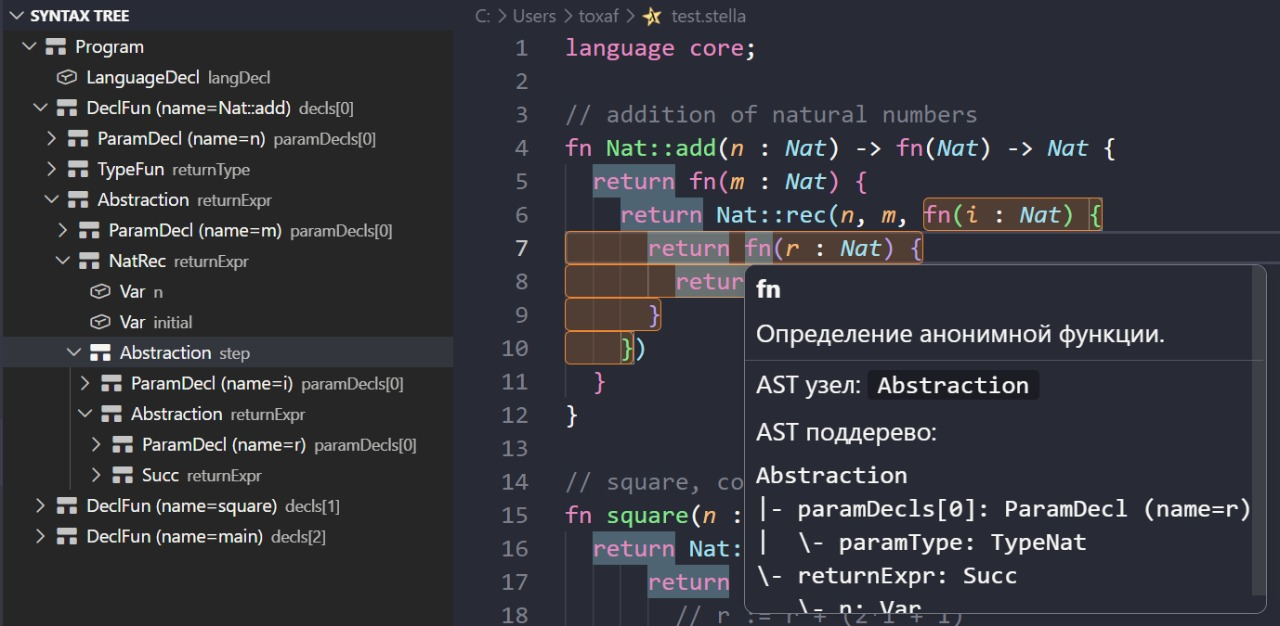
\includegraphics[width=\textwidth]{figs/ast.jpg}
    \caption[Synchronized AST view for a Stella function]{Synchronized AST view for a Stella function. The selected \texttt{Abstraction} node in the tree corresponds to the highlighted nested function in the editor; the hover panel shows the node kind and a textual subtree.}
    \label{fig:ast}
\end{figure}

\section{Scope and Context View}

The server constructs scope frames from ancestors of the active AST node. Separate handlers collect program declarations, function parameters, local declarations, \texttt{let} bindings, recursive bindings, and variables introduced by patterns. Type labels are obtained from explicit annotations or inferred type information when available.

The client renders each frame as a collapsible group and each binding as a child item. Figure~\ref{fig:context} shows three frames: a lambda frame, a function frame, and the program frame. This presentation makes it possible to distinguish the local parameter \texttt{m}, the outer function parameter \texttt{n}, and globally declared functions.

\begin{figure}[htbp]
    \centering
    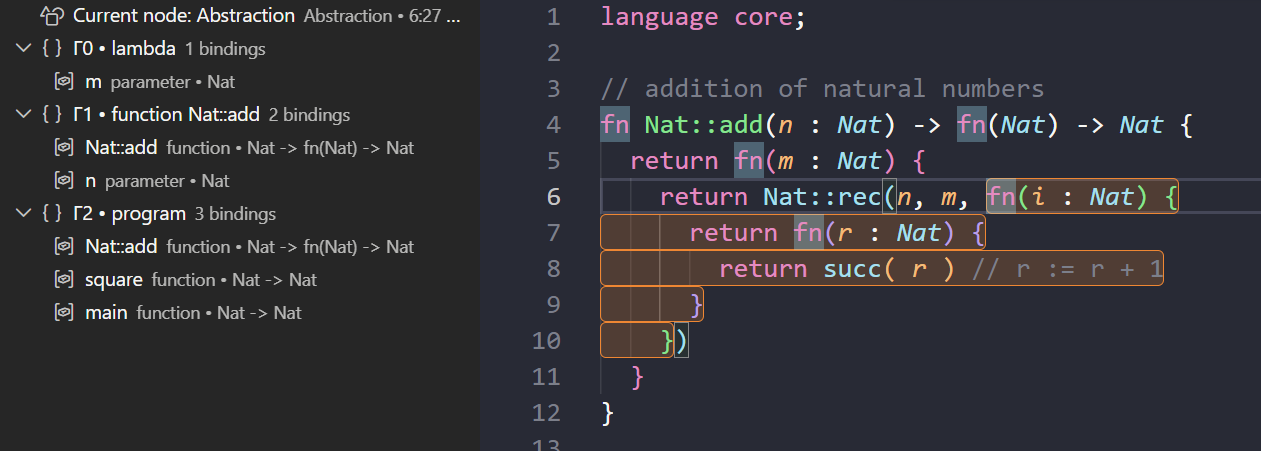
\includegraphics[width=\textwidth]{figs/context_panel.png}
    \caption[Scope and typing-context view for a nested abstraction]{Scope and typing-context view at a nested Stella abstraction. Frames $\Gamma_0$, $\Gamma_1$, and $\Gamma_2$ separate bindings introduced by the lambda, the enclosing function, and the program; each binding includes its role and type.}
    \label{fig:context}
\end{figure}

\section{Type Derivation View}

The server builds a recursive \texttt{TypeDerivationNode}. A node contains a rule name, a conclusion, zero or more premises, a source range, expression text, inferred type, and context text. The client renders premises above a horizontal rule and the conclusion below it.

Figure~\ref{fig:derivation} shows a derivation for nested abstractions ending in \texttt{succ(r)}. The path includes \textsc{T-Var}, \textsc{T-Succ}, and two \textsc{T-Abs} applications. A click on any rule sends its range back to the extension and highlights the corresponding source fragment.

\begin{figure}[htbp]
    \centering
    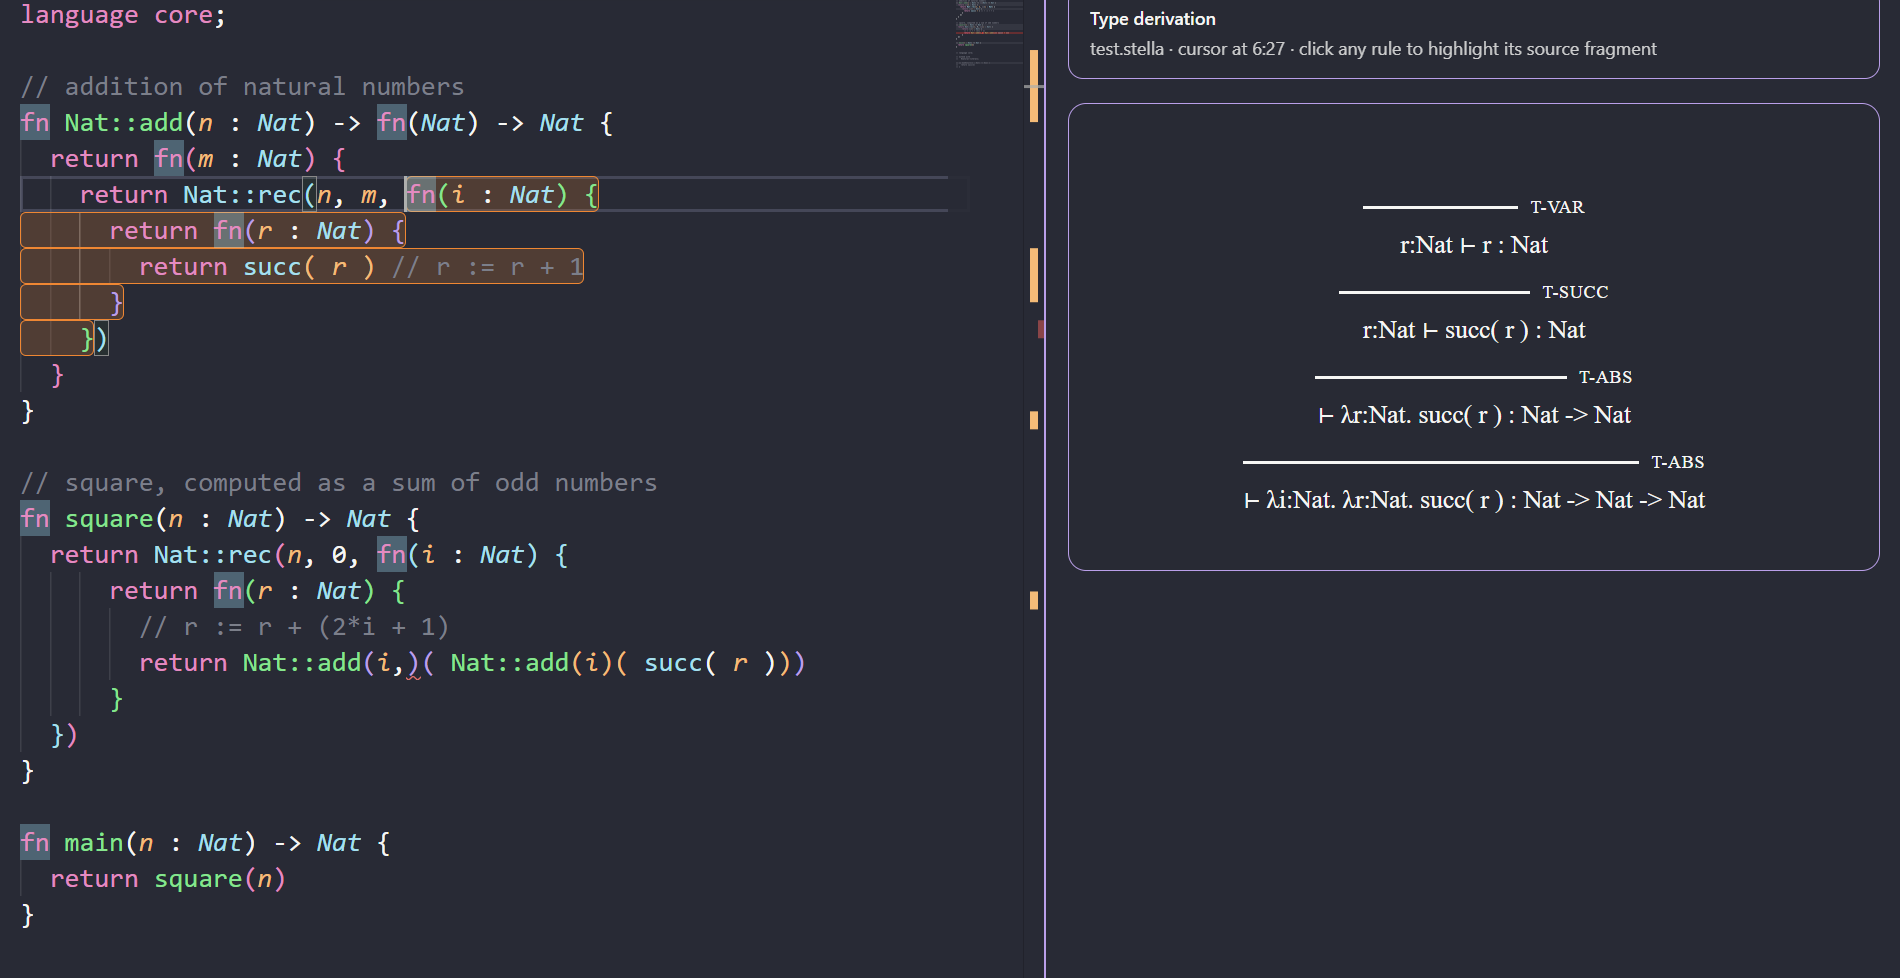
\includegraphics[width=\textwidth]{figs/derivation_tree.png}
    \caption[Interactive type derivation for nested abstractions]{Interactive type derivation for nested Stella abstractions. Premises are placed above rule lines, conclusions below them, and the editor highlights the source fragment associated with the selected derivation step.}
    \label{fig:derivation}
\end{figure}

\section{Type-Error Trace}

The error-trace command first chooses a type-related diagnostic near the cursor. Parser diagnostics and token-expectation messages are filtered out. The server then builds a sequence of related expressions and checks. Each step contains a rule name, judgment, explanation, type information, and source range.

Figure~\ref{fig:error-trace} shows a function declared to return \texttt{Bool} whose body \texttt{succ(n)} has type \texttt{Nat}. The first card states the function contract, and the next card identifies the computed body type. The red border distinguishes the conflict path from an ordinary derivation.

\begin{figure}[htbp]
    \centering
    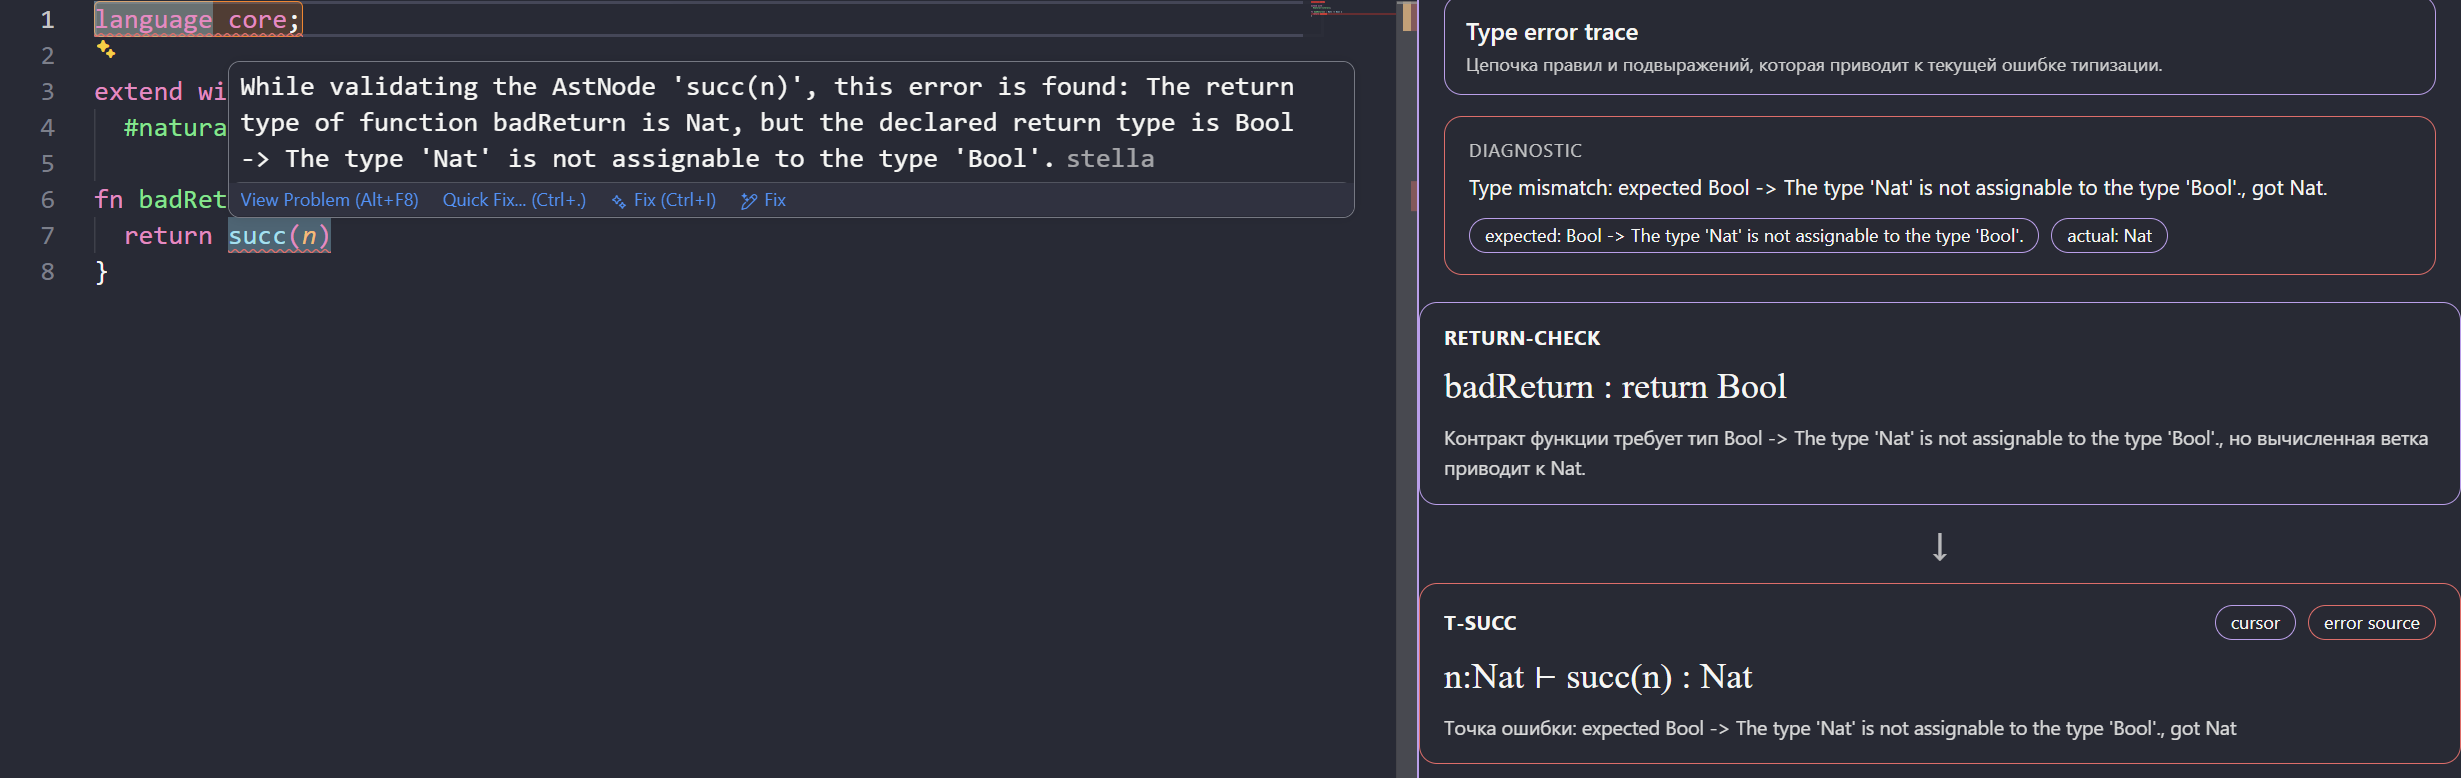
\includegraphics[width=\textwidth]{figs/error_trace.png}
    \caption[Reverse trace for a return-type mismatch]{Reverse trace for a return-type mismatch. The trace connects the declared \texttt{Bool} result of \texttt{badReturn} with the \textsc{T-Succ} judgment that gives \texttt{succ(n)} type \texttt{Nat}; the conflicting source expression is highlighted.}
    \label{fig:error-trace}
\end{figure}

\section{Type Dependency Graph}

The dependency-graph server handler creates nodes for the selected expression and relevant functions, parameters, bindings, cases, and child expressions. Nodes are assigned layers so that dependencies are displayed from left to right. Directed edges are labeled according to their role in type checking.

For a function application, the graph connects the called function and each argument to the application. For a conditional expression, it creates edges for the condition, the \texttt{then} branch, and the \texttt{else} branch. For a \texttt{let} expression, the value flows into its binding, and references to that binding flow into later expressions. The enclosing function is connected through a \texttt{return} relation.

Figure~\ref{fig:dependency-graph} illustrates the graph structure on a simplified argument-mismatch example. The actual webview uses the same logical model, but renders the nodes as clickable elements and applies visual conflict styling to the marked relation.

\begin{figure}[htbp]
    \centering
    \[
    \begin{array}{ccc}
        \texttt{takesNat : Nat -> Nat} & \xrightarrow{\texttt{callee}} & \texttt{takesNat(flag)} \\[0.8em]
        \texttt{flag : Bool} & \xrightarrow{\texttt{argument/conflict}} & \texttt{takesNat(flag)}
    \end{array}
    \]
    \caption[Type dependency graph for an argument mismatch]{Simplified type dependency graph for an argument mismatch. The application depends on the called function and on the argument expression; the argument edge is marked as conflicting because \texttt{flag} has type \texttt{Bool}, while \texttt{takesNat} expects \texttt{Nat}.}
    \label{fig:dependency-graph}
\end{figure}

The server compares available type labels with rule expectations. A mismatching argument or incompatible pair of branches sets \texttt{isConflict} on the corresponding nodes and edges. The webview uses the Visual Studio Code error color for these elements. Clicking a graph node reveals its source range, so the graph remains connected to the selected program.

\section{Evolution of the Prototype}

The implementation was developed in several iterations.

The first iteration exposed the AST and synchronized it with the cursor. This established stable node identifiers and source ranges. The second iteration added scope information. An initial flat list of names was replaced with nested frames after it became clear that a flat list did not explain where a binding originated.

The third iteration introduced the type derivation tree. The first version repeated a large context in each judgment and sometimes stopped decomposition at expressions that were still too complex. The displayed context was then reduced to bindings relevant to a subexpression, and additional expression cases were decomposed into premises. This change reduced repeated context and increased the number of displayed derivation steps, although its effect on human task performance was not measured.

The fourth iteration added reverse error tracing. Early output included parser diagnostics, which produced long token-expectation messages unrelated to typing. Diagnostic filtering and shorter explanations were added to keep the trace focused on type conflicts.

The final iteration added the type dependency graph. This view complements the derivation tree: the derivation emphasizes formal rules, while the graph emphasizes relations and conflict propagation. The iterations show that the implementation evolved from structural navigation toward semantic explanation, while reusing the same source-range and custom-request infrastructure.

\section{Chapter Summary}

The implementation provides five separate but coordinated visualizations. Semantic data is computed on the server, transferred through typed custom LSP requests, and rendered by the Visual Studio Code client. The next chapter evaluates whether these components satisfy the observable requirements defined in Chapter~\ref{chap:design}.



